% 第一章 引言
\chapter{引言}

\section{选题背景与意义}

传统冯诺依曼计算架构存在存储器与处理器物理隔离的瓶颈，数据频繁搬运导致了高昂的延迟与能耗成本。随着晶体管特征尺寸逼近物理极限，依赖缩小器件尺寸来延续摩尔定律的路径面临严重的热功耗挑战。为突破现有算力限制，存算一体架构与神经形态计算成为近期的研究热点。拓扑磁性材料因具备非易失性、驱动能耗低以及易于与主流半导体工艺集成等特点，被视为实现新型存算器件的物理载体。

在现有的磁性拓扑结构中，二维斯格明子因自旋构型简单且具备成熟的实验观测条件而受到广泛关注\cite{gobel2021beyond}。但二维体系在信息存储密度与动力学调控空间上存在局限。斯格明子的面内几何尺度限制了器件的进一步集成，且其运动轨迹被约束于薄膜面内。此外二维斯格明子对薄膜几何边界与各向异性参数较为敏感，导致其拓扑稳定性易受影响。

相较于二维体系，三维磁性拓扑准粒子霍普夫子在空间维度上扩展了设计的自由度\cite{gobel2021beyond,guslienko2024review}。霍普夫子具有由非零 Hopf 指数定义的三维自旋纽结构型，该构型受拓扑保护机制作用，能够抵抗外界环境的微小扰动。由于额外引入了轴向自由度，霍普夫子展现出与二维斯格明子不同的三维动力学行为，这为开发高密度存储和类脑计算器件提供了底层物理机制。

斯格明子与霍普夫子在自旋结构上的对比如\cref{fig:skyrmion-hopfion-compare}所示。

\begin{figure}[htbp]
  \centering
  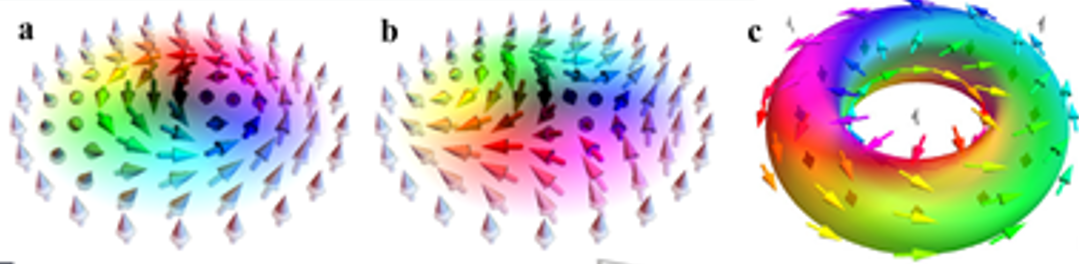
\includegraphics[width=0.85\textwidth]{figures/fig1-1_skyrmion_vs_hopfion.png}
  \caption{二维斯格明子与三维霍普夫子的自旋构型对比。(a) N\'{e}el 型斯格明子，自旋沿径向从中心向外逐渐翻转；(b) Bloch 型斯格明子，自旋沿切向形成旋涡状排布；(c) 霍普夫子，其自旋沿环面方向连续扭转形成甜甜圈状三维纽结构型，颜色色相映射面内磁化方向。}
  \label{fig:skyrmion-hopfion-compare}
\end{figure}

从自旋结构的几何关系看，霍普夫子可以视作由笔直的斯格明子管经过 $360°$ 扭曲后首尾相接形成的三维纽结\cite{liu2020magnetic_hopfion}，其构造过程如\cref{fig:skyrmion-to-hopfion}所示。这一图像有助于直观理解霍普夫子相对于二维旋涡结构的几何复杂性与拓扑来源。

\begin{figure}[htbp]
  \centering
  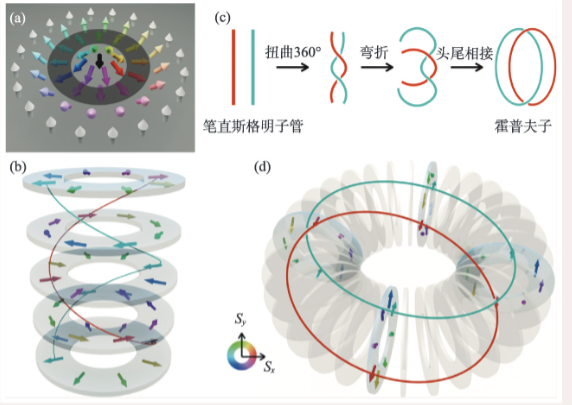
\includegraphics[width=0.85\textwidth]{figures/fig1-2_skyrmion_to_hopfion.png}
  \caption{斯格明子与霍普夫子的几何联系。(a) 斯格明子自旋结构的顶视图; (b) 沿 $z$ 方向堆叠的斯格明子管; (c) 由笔直斯格明子管扭曲 $360°$ 后弯折并首尾相接，即可构造出霍普夫子; (d) 霍普夫子中两条不同自旋方向的前像（preimage）闭环在三维空间内相互缠绕\cite{liu2020magnetic_hopfion}。}
  \label{fig:skyrmion-to-hopfion}
\end{figure}

\section{国内外研究动态}

霍普夫子（Hopfion）一词源自德国数学家海因茨·霍普夫（Heinz Hopf），其 1931 年提出的 Hopf 映射\cite{hopf1931abbildungen}定义了从 $S^3$ 到 $S^2$ 的连续映射，由此导出的整数拓扑不变量，也称为Hopf 指数，构成该类三维拓扑构型的数学分类基础。经典场论率先在 1997 年证明了纽结状拓扑构型能以稳定有限能量解的形式存在\cite{faddeev1997knots}，此后这一概念逐步从高能物理转移至凝聚态磁学体系。较早的理论工作论证了非中心对称磁性纳米结构中静态 Hopf 孤子的存在性\cite{tai2018static}，从而奠定了该拓扑构型在固态磁性材料中得以实现的理论基础。随后，磁性多层膜体系被用于 霍普夫子 的构建与实验观测\cite{kent2021creation}。2023 年，已有工作利用电子全息术在立方手性磁体中实现了稳定 霍普夫子 环的直接成像\cite{zheng2023hopfion}，该成果在实验层面具有里程碑式的意义。

结构稳定性是拓扑粒子应用于逻辑器件的前提。目前学术界对霍普夫子稳定性的探讨主要集中于包含 Dzyaloshinskii-Moriya 相互作用（DMI）的手性磁体体系\cite{guslienko2024review}。研究人员通过解析推导确定了其理论自旋构型\cite{sutcliffe2018hopfions}，并利用微磁学仿真论证了纳米几何边界的束缚能力\cite{liu2018binding}以及体块结构中的椭圆稳定性条件\cite{metlov2025elliptical}。配合 MnGe 与 FeGe 体系中的观测实验\cite{zheng2023hopfion,yu2023realization}，基于 DMI 体系的霍普夫子稳定参数空间已得到充分验证。

与手性磁体相比，阻挫交换铁磁体系中的拓扑稳定性研究尚处于探索阶段。虽然理论计算指出阻挫交换作用同样具备稳定三维拓扑构型的物理能力\cite{sallermann2023stability}，并初步分析了霍普夫子在该体系下的有限寿命与坍塌模式\cite{lobanov2023lifetime}，但针对该物理框架的系统性参数扫描与稳态规律分析仍有待补充。本研究的稳定性数值实验即选定阻挫交换铁磁模型作为计算基底。

动力学特性是决定拓扑磁结构器件应用潜力的核心要素。在接触式电流驱动（如自旋转移力矩 STT）机制下，理论推导证明铁磁体内 Bloch 型与 N\'{e}el 型霍普夫子能够沿电流方向发生无霍尔偏转的直线运动\cite{wang2019current}，且其回旋矢量与 Hopf 指数存在定量约束关系\cite{liu2020three}。相关微磁学特性也在 FeGe 材料中得到了实验证实，分数霍普夫子在较低电流密度下即可起动，其运动方向受 Hopf 指数符号调控\cite{yu2023realization}。除常规线性响应外，涌现磁多极矩构型还为霍普夫子提供了非线性动力学通道\cite{liu2022emergent}。在非接触式的自旋波（Magnon）驱动领域，现有研究已确认自旋波可有效推动二维斯格明子及其变体\cite{ding2015motion,huang2023transient,shen2018skyrmionium}。针对三维霍普夫子，理论预测其能够引发磁振子霍尔效应与磁振子聚焦现象\cite{saji2023magnonic}，且反铁磁霍普夫子在调节自旋波散射方面具备应用可行性\cite{zhang2023magnon,pershoguba2021electronic}。最新的仿真结果进一步指出，自旋波驱动在引发运动的同时可能伴随拓扑态转变\cite{souza2025topological}。另外外部磁场、自旋轨道力矩（SOT）与电场等激励手段也能引发霍普夫子晶格周期调节\cite{metlov2025control}、高阶态重组\cite{kasai2025sot}以及三维拓扑轨道霍尔效应\cite{goebel2025orbital}。

尽管目前关于霍普夫子静态构型与拓扑性质的研究已相对完备，但关于其在自旋波非接触激励下的动力学机制仍缺乏系统性的数值论证。这一理论空缺限制了三维拓扑磁结构在低功耗逻辑器件中的应用拓展。本研究据此依托微磁学数值模拟方法，考察阻挫交换铁磁体系中霍普夫子的稳态条件与自旋波驱动下的响应规律，并评估该物理机制映射至神经形态计算概念架构的可行性。


\section{本文的研究内容与章节安排}

全文的研究内容与章节组织如下：

第一章阐述选题背景，梳理霍普夫子稳定性及动力学方面的研究现状，明确研究目标。第二章介绍微磁学基本理论、Landau-Lifshitz-Gilbert 动力学方程及霍普夫子拓扑性质，为后续数值计算奠定理论基础。第三章提出基于局域旋转矩阵与环面坐标映射的自旋构型初始化方法，开发支持任意拓扑荷的三维可视化工具。第四章针对阻挫交换铁磁模型，分析霍普夫子的能量弛豫演化过程，并探讨磁晶各向异性对结构稳定性的影响。第五章研究自旋波驱动下的动力学规律，考察极化依赖特性、频率响应谱及 srcX/srcZ 方向互补格局，并提出对应的双向轴向调控方案。第六章提取上述微磁学动力学特征，建立其与生物神经元核心功能的映射关系，探讨基于自旋波信息载体的神经形态器件架构。第七章对研究工作进行总结，归纳主要结论并指出未来拓展方向。
